\section{L'interfaccia}

L'interfaccia utente del sistema è stata rivisitata ed adattata alle nuove esigenze. 

\begin{figure*}
\begin{center}
\centering
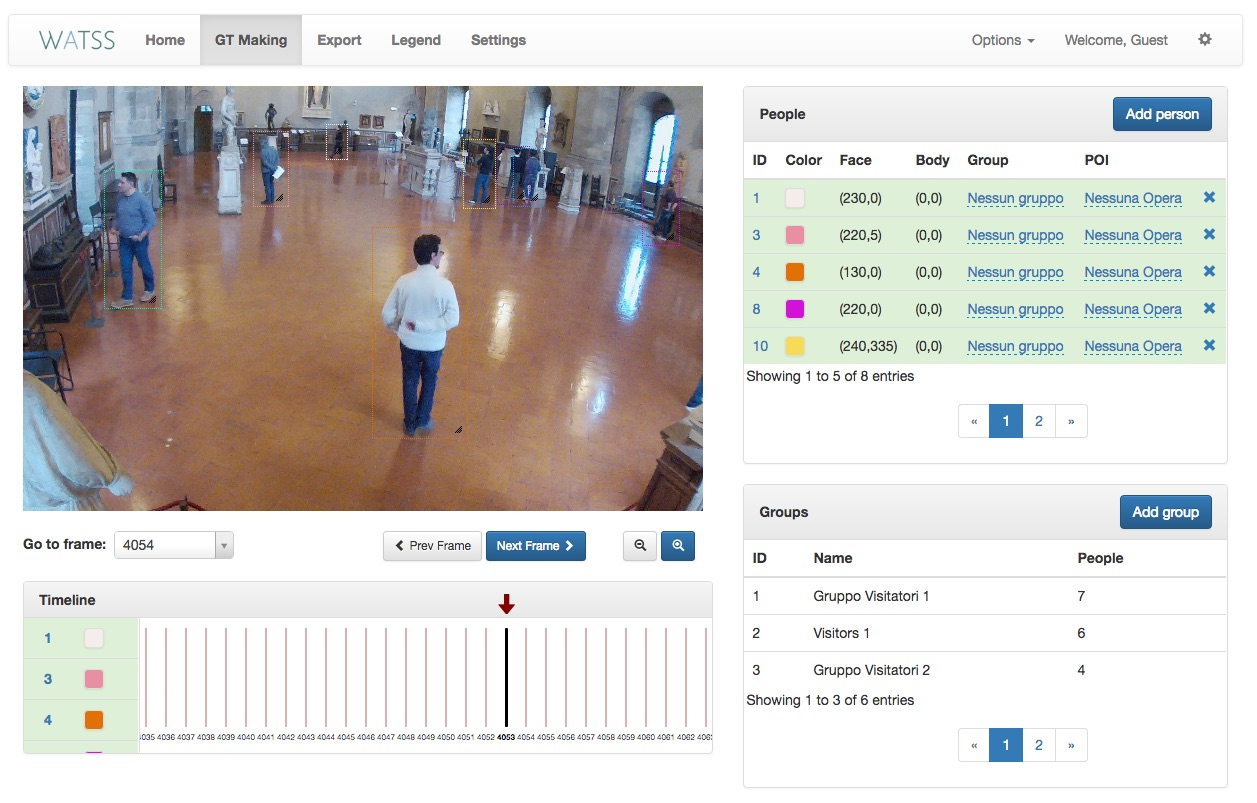
\includegraphics[width=1\linewidth]{images/watss-gui.jpg}
  \label{fig:watss-gui}
  \caption{Interfaccia utente del tool WATSS}
\end{center}
\end{figure*}

La parte principale è costituita dal frame video su cui andremo ad aggiungere annotazioni e visualizzare quelle già esistenti.
I due pannelli laterali per le persone e gruppi presenti nella scena sono stati organizzati in modo tale da consentirne una rapida navigazione ed uso. Come nella precedente versione dell'interfaccia, il pannello \emph{People} mostra la lista delle annotazioni presenti nel frame visualizzato, ordinate in base all'identificativo delle persone. Per ciascuna persona viene mostrato il \emph{gaze }del corpo e della faccia, il \emph{gruppo di appartenenza} ed il \emph{punto di interesse} presso cui si trovano. 

\subsection{Inserimento di una annotazione}

Tramite il pulsante \emph{Add person} presente nel pannello delle annotazioni è possibile aggiungere una nuova annotazione al frame. 

\begin{figure}[h]
\centering
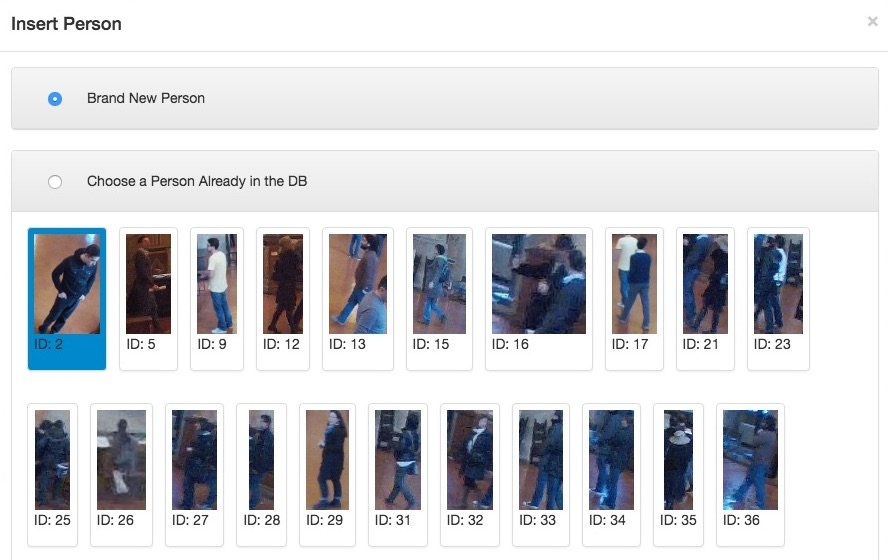
\includegraphics[width=0.8\linewidth]{images/add-person.jpg}
  \caption{Aggiunta di una nuova annotazione}
  \label{fig:addperson}
\end{figure}

Come mostrato in Figura \ref{fig:addperson}, in fase di creazione è possibile indicare se si vuole aggiungere un'annotazione rappresentante una nuova identità ancora non presente nel database oppure se si vuole aggiungere una nuova istanza di un'identità già presente e di cui viene mostrato un \emph{avatar}.

Una volta selezionata l'opzione desiderata, la fase di creazione è diversa in base all'attivazione della \emph{geometria della scena} o meno. Per l'attivazione e la disattivazione della geometria è sufficiente spuntare l'opzione presente nel menù \emph{Options} della barra principale di navigazione.

In caso di geometria della scena \emph{disattivata} la nuova annotazione verrà creata con la tecnica \emph{click and drag}: l'utente clicca nel frame nel punto in cui vuole iniziare la sua selezione e tiene premuto spostando il mouse finchè la bounding box visualizzata non è della dimensione desiderata. A quel punto, rilasciando il click, la bounding box verrà inserita nella scena.

Se invece è attiva la geometria, questa verrà sfruttata per stimare l'altezza di una persona presente nella scena in base alla sua posizione nella stessa. La bounding box verrà automaticamente attaccata al puntatore del mouse e, muovendosi nella scena, sarà ridimensionata in base alla sua posizione. Una volta scelta la posizione, per effettuare l'inserimento sarà sufficiente effettuare un click nel punto desiderato. 

In entrambi i casi, la procedura di inserimento può essere interrotta premendo il tasto \emph{ESC}.

\subsection{Modifica di una annotazione}

E' stata inoltre migliorata la fase di modifica delle annotazioni presenti. Le bounding box sono ora trascinabili e ridimensionabili mediante il mouse. 

Sia in fase di creazione che di modifica è ora possibile effettuare uno zoom del frame così da poter raffinare delle annotazioni. Questo si è reso necessario soprattutto per quanto riguarda oggetti e persone molto piccoli nella scena. 

Selezionando una bounding box è infine possibile ridimensionarla semplicemente mediante la rotellina del mouse, consentendo una rapida scalatura del rettangolo definito.

\subsection{La timeline}



